
\section*{5.1 The quantum Fourier transform}

% One of the most useful ways of solving a problem in mathematics or computer science is to transform it into some other problem for which a solution is known. There are a few transformations of this type which appear so often and in so many different contexts that the transformations are studied for their own sake. 

% A great discovery of quantum computation has been that some such transformations can be computed much faster on a quantum computer than on a classical computer. One such transformation is the discrete Fourier transform.

\subsection{Quantum Fourier Transform}

In the usual mathematical notation, the \textbf{discrete Fourier transform} takes as input a vector of complex numbers, $x_{0}, \ldots, x_{N-1}$ where the length $N$ of the vector is a fixed parameter. It outputs the transformed data, a vector of complex numbers $y_{0}, \ldots, y_{N-1}$, defined by
\begin{equation*}
y_{k} \equiv \frac{1}{\sqrt{N}} \sum_{j=0}^{N-1} x_{j} e^{2 \pi i j k / N}, \quad \forall k = 0,\dots,N-1.
\tag{5.1}
\end{equation*}
Notice! Be careful not to confuse imaginary $i$ with index $i$.

The quantum Fourier transform is exactly the same transformation, although the conventional notation for the quantum Fourier transform is somewhat different. 

\begin{definition}[quantum Fourier transform]
    The quantum Fourier transform on an orthonormal basis $|0\rangle, \ldots,|N-1\rangle$ is defined to be a linear operator with the following action on the basis states,
\begin{equation*}
|j\rangle \longrightarrow \frac{1}{\sqrt{N}} \sum_{k=0}^{N-1} e^{2 \pi i j k / N}|k\rangle, \quad \forall j = 0,\dots,N-1. \tag{5.2}
\end{equation*}
\end{definition}

Equivalently, the action of quantum Fourier transform on an arbitrary state may be written
\begin{equation*}
\sum_{j=0}^{N-1} x_{j}|j\rangle \longrightarrow \sum_{k=0}^{N-1} y_{k}|k\rangle \tag{5.3}
\end{equation*}
where the amplitudes $y_{k}$ are the discrete Fourier transform of the amplitudes $x_{j}$.  Let $U$ denote the quantum Fourier transform defined above. To show (5.3), we have
\begin{align*}
    U(\sum_{j=0}^{N-1} x_{j}|j\rangle) &= \sum_{j=0}^{N-1} x_{j} U|j\rangle \\
    &= \sum_{j=0}^{N-1} x_{j} \left(\frac{1}{\sqrt{N}} \sum_{k=0}^{N-1} e^{2 \pi i j k / N}|k\rangle \right) \\
    &= \frac{1}{\sqrt{N}} \sum_{j=0}^{N-1}  \sum_{k=0}^{N-1} x_{j} e^{2 \pi i j k / N}|k\rangle \\
    &= \frac{1}{\sqrt{N}} \sum_{k=0}^{N-1} \sum_{j=0}^{N-1}   x_{j} e^{2 \pi i j k / N}|k\rangle \\
    &= \sum_{k=0}^{N-1} \left(\frac{1}{\sqrt{N}}  \sum_{j=0}^{N-1}   x_{j} e^{2 \pi i j k / N}|k\rangle \right)\\
    &= \sum_{k=0}^{N-1} y_{k}|k\rangle. \\
\end{align*}

This transformation is a unitary transformation, and thus can be implemented as the dynamics for a quantum computer. 

\begin{theorem}
    The quantum Fourier transform is a unitary transformation.
\end{theorem}

\begin{proof}
Let $U$ denote the quantum Fourier transform defined above. Taking any two vectors $|j\rangle, |j^{\prime}\rangle$ from the orthonormal basis $|0\rangle, \ldots,|N-1\rangle$, we have 
$$
U|j\rangle=\frac{1}{\sqrt{N}} \sum_{k=0}^{N-1} e^{2 \pi i j k / N}|k\rangle,
U|j^{\prime}\rangle=\frac{1}{\sqrt{N}} \sum_{k^{\prime}=0}^{N-1} e^{2 \pi i j^{\prime} k / N}|k^{\prime}\rangle,
$$
and
$$
\left\langle j^{\prime}\left|U^{\dagger} U\right| j\right\rangle=\frac{1}{N} \sum_{k=0}^{N-1} e^{2 \pi i\left(j-j^{\prime}\right) k / N}.
$$
Consider the case 1 that $\Delta j=j-j^{\prime}=0,$ then $\left\langle j^{\prime}\left|U^{\dagger} U\right| j\right\rangle=1.$
Consider the case 2 that $\Delta j=j-j^{\prime} \neq 0$ but $\Delta j  \in \mathbb{Z}$, then
\begin{align}
\left\langle j^{\prime}\left|U^{\dagger} U\right| j\right\rangle = & \frac{1}{N} \sum_{k=0}^{N-1} r^k \quad \left(r:=e^{2 \pi i \Delta j / N}\right) \\
= & \frac{1}{N} \cdot \frac{1-r^N}{1-r} \\ 
= & \frac{1}{N} \cdot  \frac{1-e^{2 \pi i \Delta j}}{1-r}=0.
\end{align}
\end{proof}

% Exercise 5.1: Give a direct proof that the linear transformation defined by Equation (5.2) is unitary.

\begin{exercise}
    Exercise 5.2: Explicitly compute the Fourier transform of the $n$ qubit state $|00 \ldots 0\rangle$. Actually, this is very easy. If we use the decimal numbering, then $|00 \ldots 0\rangle$ is $|j\rangle$ with $j=0$. Then, we obtain $\frac{1}{\sqrt{N}} \sum_{k=0}^{N-1}|k\rangle$.
\end{exercise}

In the following, we take $N=2^{n}$, where $n$ is some integer, and the basis $|0\rangle, \ldots, \mid 2^{n}-$ $1\rangle$ is the computational basis for an $n$ qubit quantum computer. It is helpful to write the state $|j\rangle$ (thus, $j=0,1,\dots,2^n-1$) using the binary representation 
$$
j=j_{1} j_{2} \ldots j_{n}.
$$
More formally, $j=j_{1} 2^{n-1}+j_{2} 2^{n-2}+\cdots+j_{n} 2^{0}$. Note that $j=\sum_{l=1}^n j_l 2^{n-l}.$

It is also convenient to adopt the notation $0 . j_{l} j_{l+1} \ldots j_{m}$ to represent the  binary fraction $j_{l} / 2+j_{l+1} / 4+\cdots+j_{m} / 2^{m-l+1}.$ % 请另行参考资料 binary fraction

\begin{theorem}
    With a little algebra the quantum Fourier transform can be given the following useful \textbf{(tensor) product representation}:
\begin{equation*}
\left|j_{1}, \ldots, j_{n}\right\rangle \rightarrow \frac{\left(|0\rangle+e^{2 \pi i 0 \cdot j_{n}}|1\rangle\right)\left(|0\rangle+e^{2 \pi i 0 \cdot j_{n-1} j_{n}}|1\rangle\right) \cdots\left(|0\rangle+e^{2 \pi i 0 \cdot j_{1} j_{2} \cdots j_{n}}|1\rangle\right)}{2^{n / 2}} \tag{5.4}
\end{equation*}
This product representation is so useful that you may even wish to consider this to be the definition of the quantum Fourier transform. 
\end{theorem}

As we explain shortly this representation allows us to construct an efficient quantum circuit computing the Fourier transform, and provides insight into algorithms based upon the quantum Fourier transform.

The equivalence of the product representation (5.4) and the definition (5.2) follows from some elementary algebra:
\begin{align*}
|j\rangle & \rightarrow \frac{1}{2^{n / 2}} \sum_{k=0}^{2^{n}-1} e^{2 \pi i j k / 2^{n}}|k\rangle \quad (\text{decimal number } k) \tag{5.5}\\
& =\frac{1}{2^{n / 2}} \sum_{k_{1}=0}^{1} \cdots \sum_{k_{n}=0}^{1} e^{2 \pi i j\left(\sum_{l=1}^{n} k_{l} 2^{-l}\right)}\left|k_{1} k_{2} \ldots k_{n}\right\rangle  \quad (\text{binary number } k = \sum_{l=1}^n k_l 2^{n-l})\tag{5.6}\\
& =\frac{1}{2^{n / 2}} \sum_{k_{1}=0}^{1} \ldots \sum_{k_{n}=0}^{1} \bigotimes_{l=1}^{n} e^{2 \pi i j k_{l} 2^{-l}}\left|k_{l}\right\rangle  \tag{5.7}\\
& =\frac{1}{2^{n / 2}} \bigotimes_{l=1}^{n}\left[\sum_{k_{l}=0}^{1} e^{2 \pi i j k_{l} 2^{-l}}\left|k_{l}\right\rangle\right]  \tag{5.8}\\
& =\frac{1}{2^{n / 2}} \bigotimes_{l=1}^{n}\left[|0\rangle+e^{2 \pi i j 2^{-l}}|1\rangle\right]  \quad (\text{since either 0 or 1 for } k_{l})  \tag{5.9}\\
& =\frac{\left(|0\rangle+e^{2 \pi i 0. j_{n}}|1\rangle\right)\left(|0\rangle+e^{2 \pi i 0. j_{n-1} j_{n}}|1\rangle\right) \cdots\left(|0\rangle+e^{2 \pi i 0. j_{1} j_{2} \cdots j_{n}}|1\rangle\right)}{2^{n / 2}} . \tag{5.10}
\end{align*} 
For the last equality above, let consider the case $l=1$ in (5.9). Then we have
\begin{align*}
    j \cdot 2^{-1} 
    &=(j_{1} 2^{n-1}+j_{2} 2^{n-2}+\cdots+j_{n} 2^{0})\cdot 2^{-1}\\
    &=\underbrace{j_{1} 2^{n-2}+\cdots+j_{n-1} 2^{0}}_{\text{integer part of $j$, we denote it by $I$}} +\underbrace{j_{n} 2^{-1}}_{\text{fraction part of $j$, and it is $0.j_n$}} \\
    &=I + 0.j_n
\end{align*}
and $e^{2 \pi i  j 2^{-1}}=e^{2 \pi i (I + 0.j_n)}=e^{2 \pi i (0.j_n)}$. Let consider the case $l=2$ in (5.9). Then we have
\begin{align*}
    j \cdot 2^{-2} 
    &=(j_{1} 2^{n-1}+j_{2} 2^{n-2}+\cdots+j_{n} 2^{0})\cdot 2^{-2}\\
    &=\underbrace{j_{1} 2^{n-3}+\cdots+j_{n-2} 2^{0}}_{\text{integer part of $j$, we denote it by $I$}} +\underbrace{j_{n-1} 2^{-1}+ j_{n} 2^{-2}}_{\text{fraction part of $j$, and it is $0.j_{n-1}j_n$}} \\
    &=I + 0.j_{n-1}j_n
\end{align*}
and $e^{2 \pi i  j 2^{-2}}=e^{2 \pi i (I + 0.j_{n-1}j_n)}=e^{2 \pi i (0.j_{n-1}j_n)}$. For larger $l$, we have the same conclusion.

\subsection{Efficient circuit for the quantum Fourier transform}

\begin{figure}     
\centering
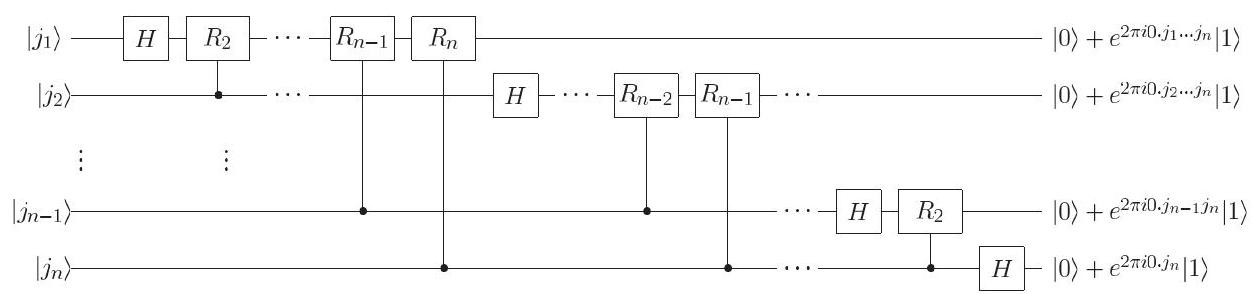
\includegraphics[width=1\linewidth]{Images/2024_05_17_6977ce60de6fd27aef98g-253}
\caption{Figure 5.1. Efficient circuit for the quantum Fourier transform. This circuit is easily derived from the product representation (5.4) for the quantum Fourier transform. Not shown are swap gates at the end of the circuit which reverse the order of the qubits, or normalization factors of $1 / \sqrt{2}$ in the output.}
\end{figure}

The product representation (5.4) makes it easy to derive an efficient circuit for the quantum Fourier transform. Such a circuit is shown in Figure 5.1. 

In Figure 5.1, the gate $R_{k}$ denotes the unitary transformation
\begin{equation*}
R_{k} \equiv\left[\begin{array}{cc}
1 & 0  \tag{5.11}\\
0 & e^{2 \pi i / 2^{k}}
\end{array}\right], \quad \forall k = 1,2,\dots,n.
\end{equation*}
Note that $R_{k} |0\rangle = |0\rangle$ for all $k.$ When $k=1,$ $R_{1} |1\rangle = e^{2 \pi i\cdot 2^{-1}}|1\rangle = e^{2 \pi i\cdot (0.1)_2}|1\rangle$. When $k=2,$ $R_{2} |1\rangle = e^{2 \pi i\cdot 2^{-2}}|1\rangle = e^{2 \pi i\cdot (0.01)_2}|1\rangle.$ Similarly, for $k=1,2,\dots,n,$ one has
$$
R_{k} |1\rangle = e^{2 \pi i\cdot (0.0 \dots 1)_2}|1\rangle
$$
where the $(0.0 \dots \underbrace{1}_{k-th})_2=2^{-k}.$

To see that the pictured circuit computes the quantum Fourier transform, consider what happens when the state $\left|j_{1} \ldots j_{n}\right\rangle$ is input. 

Applying the Hadamard gate to the first bit produces the state
\begin{equation*}
|\psi_1\rangle:=\frac{1}{2^{1 / 2}}\left(|0\rangle+e^{2 \pi i 0 \cdot j_{1}}|1\rangle\right)\left|j_{2} \ldots j_{n}\right\rangle. \tag{5.12}
\end{equation*}
In above, note that $0.j_1=0$ if $j_1=0$ and $0.j_1=\frac{1}{2}$ if $j_1=1.$ Thus, $e^{2 \pi i 0 . j_{1}}=-1$ when $j_{1}=1$, and $e^{2 \pi i 0 . j_{1}}=1$  when $j_{1}=0.$

Recall that applying the \textit{controlled-$R_{2}$ gate} to $|x_1 x_2 \rangle$ yields $(R_{2}^{x_2}|x_1\rangle) |x_2 \rangle$ when the controlled qubit is $x_2$ and target qubit is $x_1$, where $x_1,x_2=0,1.$ Thus, applying the controlled-$R_{2}$ gate to $|\psi_1\rangle$ produces the state
\begin{align*}
&\frac{1}{2^{1 / 2}} \left( R_{2}^{j_2} \left(|0\rangle+e^{2 \pi i 0 \cdot j_{1}}|1\rangle\right) \right) \left|j_{2} \ldots j_{n}\right\rangle \\
=&\frac{1}{2^{1 / 2}}\left(R_{2}^{j_2} |0\rangle+e^{2 \pi i 0 \cdot j_{1} j_{2}}\cdot R_{2}^{j_2} |1\rangle\right)\left|j_{2} \ldots j_{n}\right\rangle \\
=&\frac{1}{2^{1 / 2}}\left(|0\rangle+e^{2 \pi i 0 \cdot j_{1} j_{2}}|1\rangle\right)\left|j_{2} \ldots j_{n}\right\rangle.     \tag{5.13}
\end{align*}
It is easy to check the above equality holds for both $j_2=0$ and $j_2=1.$ 

We continue applying the \textit{controlled-$R_{3}, R_{4}$ through $R_{n}$ gates}, each of which adds an extra bit to the phase of the co-efficient of the first $|1\rangle$. At the end of this procedure we have the state
\begin{equation*}
\frac{1}{2^{1 / 2}}\left(|0\rangle+e^{2 \pi i 0 \cdot j_{1} j_{2} \ldots j_{n}}|1\rangle\right)\left|j_{2} \ldots j_{n}\right\rangle. \tag{5.14}
\end{equation*}

Next, we perform a similar procedure on the second qubit. The Hadamard gate puts us in the state
\begin{equation*}
\frac{1}{2^{2 / 2}}\left(|0\rangle+e^{2 \pi i 0 \cdot j_{1} j_{2} \ldots j_{n}}|1\rangle\right)\left(|0\rangle+e^{2 \pi i 0 \cdot j_{2}}|1\rangle\right)\left|j_{3} \ldots j_{n}\right\rangle \tag{5.15}
\end{equation*}
and the \textit{controlled-$R_{2}$ through $R_{n-1}$ gates} yield the state
\begin{equation*}
\frac{1}{2^{2 / 2}}\left(|0\rangle+e^{2 \pi i 0 \cdot j_{1} j_{2} \ldots j_{n}}|1\rangle\right)\left(|0\rangle+e^{2 \pi i 0 \cdot j_{2} \ldots j_{n}}|1\rangle\right)\left|j_{3} \ldots j_{n}\right\rangle. \tag{5.16}
\end{equation*}

We continue in this fashion for each qubit, giving a final state
\begin{equation*}
\frac{1}{2^{n / 2}}\left(|0\rangle+e^{2 \pi i 0 \cdot j_{1} j_{2} \ldots j_{n}}|1\rangle\right)\left(|0\rangle+e^{2 \pi i 0 \cdot j_{2} \ldots j_{n}}|1\rangle\right) \ldots\left(|0\rangle+e^{2 \pi i 0 \cdot j_{n}}|1\rangle\right) \tag{5.17}
\end{equation*}

Swap operations (see Section 1.3.4 for a description of the circuit), omitted from Figure 5.1 for clarity, are then used to reverse the order of the qubits. After the swap operations, the state of the qubits is

\begin{equation*}
\frac{1}{2^{n / 2}}\left(|0\rangle+e^{2 \pi i 0 \cdot j_{n}}|1\rangle\right)\left(|0\rangle+e^{2 \pi i 0 \cdot j_{n-1} j_{n}}|1\rangle\right) \ldots\left(|0\rangle+e^{2 \pi i 0 \cdot j_{1} j_{2} \cdots j_{n}}|1\rangle\right) \tag{5.18}
\end{equation*}

Comparing with Equation (5.4) we see that this is the desired output from the quantum Fourier transform. 

This construction also proves that the quantum Fourier transform is unitary, since each gate in the circuit is unitary. An explicit example showing a circuit for the quantum Fourier transform on three qubits is given in Box 5.1.

\textbf{Box 5.1: Three qubit quantum Fourier transform}

For concreteness it may help to look at the explicit circuit for the three qubit quantum Fourier transform: 
\begin{figure}     
\centering
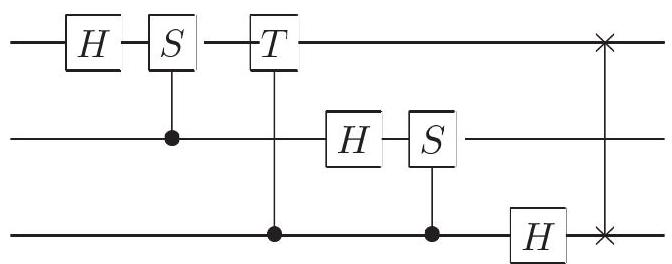
\includegraphics[width=0.75\linewidth]{Images/2024_05_17_6977ce60de6fd27aef98g-254}
\end{figure}
Recall that $S$ and $T$ are the phase and $\pi / 8$ gates. If the gate $R_{k}$ denotes the unitary transformation
\begin{equation*}
R_{k} \equiv\left[\begin{array}{cc}
1 & 0  \tag{5.11}\\
0 & e^{2 \pi i / 2^{k}}
\end{array}\right].
\end{equation*}
Then, we have $R_2=S$ and $R_3=T.$

As a matrix the quantum Fourier transform in this instance may be written out explicitly, using $\omega=e^{2 \pi i / 8}=\sqrt{i}$, as
\begin{equation*}
\frac{1}{\sqrt{8}}\left[\begin{array}{cccccccc}
1 & 1 & 1 & 1 & 1 & 1 & 1 & 1  \tag{5.19}\\
1 & \omega & \omega^{2} & \omega^{3} & \omega^{4} & \omega^{5} & \omega^{6} & \omega^{7} \\
1 & \omega^{2} & \omega^{4} & \omega^{6} & 1 & \omega^{2} & \omega^{4} & \omega^{6} \\
1 & \omega^{3} & \omega^{6} & \omega^{1} & \omega^{4} & \omega^{7} & \omega^{2} & \omega^{5} \\
1 & \omega^{4} & 1 & \omega^{4} & 1 & \omega^{4} & 1 & \omega^{4} \\
1 & \omega^{5} & \omega^{2} & \omega^{7} & \omega^{4} & \omega^{1} & \omega^{6} & \omega^{3} \\
1 & \omega^{6} & \omega^{4} & \omega^{2} & 1 & \omega^{6} & \omega^{4} & \omega^{2} \\
1 & \omega^{7} & \omega^{6} & \omega^{5} & \omega^{4} & \omega^{3} & \omega^{2} & \omega^{1}
\end{array}\right] .
\end{equation*}
You can find many materials about "matrix form of discrete Fourier transformation" on the internet.

\subsection{Discussion}

How many gates does this circuit use? 
\begin{itemize}
    \item We start by doing a Hadamard gate and $n-1$ conditional rotations on the first qubit - a total of $n$ gates.
    \item This is followed by a Hadamard gate and $n-2$ conditional rotations on the second qubit, for a total of $n-1$ gates.
    \item Continuing in this way, we see that $n+(n-1)+\cdots+1=n(n+1) / 2$ gates are required, plus the gates involved in the swaps.
    \item At most $n / 2$ swaps are required, and each swap can be accomplished using three controlled-NOT gates. 
\end{itemize}
Therefore, this circuit provides a $\Theta(n^{2})$ algorithm for performing the quantum Fourier transform.

In contrast, the best classical algorithms for computing the discrete Fourier transform on $2^{n}$ elements are algorithms such as the \textbf{Fast Fourier Transform (FFT)}, which compute the discrete Fourier transform using $\Theta\left(n 2^{n}\right)$ gates. That is, it requires exponentially more operations to compute the Fourier transform on a classical computer than it does to implement the quantum Fourier transform on a quantum computer.

Can we use the quantum Fourier transform to speed up the computation of these Fourier transforms? Unfortunately, the answer is that there is no known way to do this. 

\begin{enumerate}
    \item The problem is that the amplitudes in a quantum computer cannot be directly accessed by measurement. Thus, there is no way of determining the Fourier transformed amplitudes of the original state.
    \item Worse still, there is in general no way to efficiently prepare the original state to be Fourier transformed.
\end{enumerate}

In this and the next chapter we develop several algorithms based upon a more subtle application of the quantum Fourier transform.

\begin{exercise}
Exercise 5.3: (\textbf{Classical fast Fourier transform}) Suppose we wish to perform a Fourier transform of a vector containing $2^{n}$ complex numbers on a classical computer. Verify that the straightforward method for performing the Fourier transform, based upon direct evaluation of Equation (5.1) requires $\Theta\left(2^{2 n}\right)$ elementary arithmetic operations. Find a method for reducing this to $\Theta\left(n 2^{n}\right)$ operations, based upon Equation (5.4).
\end{exercise}

\begin{exercise}
\textbf{Exercise 5.4: Give a decomposition of the controlled-$R_{k}$ gate into single qubit and CNOT gates.}
\end{exercise}

\begin{exercise}
\textbf{Exercise 5.5: Give a quantum circuit to perform the inverse quantum Fourier transform.}
\end{exercise}

\begin{exercise}
\textbf{Exercise 5.6: (Approximate quantum Fourier transform)} The quantum circuit construction of the quantum Fourier transform apparently requires gates of exponential precision in the number of qubits used. However, such precision is never required in any quantum circuit of polynomial size. For example, let $U$ be the ideal quantum Fourier transform on $n$ qubits, and $V$ be the transform which results if the controlled-$R_{k}$ gates are performed to a precision $\Delta=1 / p(n)$ for some polynomial $p(n)$. Show that the error $E(U, V) \equiv \max _{|\psi\rangle} \|(U-V)|\psi\rangle \|$ scales as $\Theta\left(n^{2} / p(n)\right)$, and thus polynomial precision in each gate is sufficient to guarantee polynomial accuracy in the output state.
\end{exercise}

